\documentclass[12pt]{article}
\setlength\parindent{0pt}
\usepackage{fullpage}
\usepackage{amsmath}
\usepackage[margin=1.5cm]{geometry}
%\usepackage[margin=0.4in, paperwidth=13.5in, paperheight=8.4375in]{geometry}
\usepackage{graphicx}
\setlength{\parskip}{4mm}
\def\LL{\left\langle}   % left angle bracket
\def\RR{\right\rangle}  % right angle bracket
\def\LP{\left(}         % left parenthesis
\def\RP{\right)}        % right parenthesis
\def\LB{\left\{}        % left curly bracket
\def\RB{\right\}}       % right curly bracket
\def\PAR#1#2{ {{\partial #1}\over{\partial #2}} }
\def\PARTWO#1#2{ {{\partial^2 #1}\over{\partial #2}^2} }
\def\PARTWOMIX#1#2#3{ {{\partial^2 #1}\over{\partial #2 \partial #3}} }
\newcommand{\BE}{\begin{displaymath}}
\newcommand{\EE}{\end{displaymath}}
\newcommand{\BI}{\begin{itemize}}
	\newcommand{\EI}{\end{itemize}}
\newcommand{\BNE}{\begin{equation}}
\newcommand{\ENE}{\end{equation}}
\newcommand{\BEA}{\begin{eqnarray}}
\newcommand{\BS}{\bigskip}
\newcommand{\EEA}{\nonumber\end{eqnarray}}
\newcommand{\EL}{\nonumber\\}
\newcommand{\la}[1]{\label{#1}}
\newcommand{\ie}{{\em i.e.\ }}
\newcommand{\eg}{{\em e.\,g.\ }}
\newcommand{\cf}{cf.\ }
\newcommand{\etc}{etc.\ }
\newcommand{\Tr}{{\rm tr}}
\newcommand{\etal}{{\it et al.}}
\newcommand{\OL}[1]{\overline{#1}\ } % overline
\newcommand{\OLL}[1]{\overline{\overline{#1}}\ } % double overline
\newcommand{\OON}{\frac{1}{N}} % "one over N"
\newcommand{\OOX}[1]{\frac{1}{#1}} % "one over X"



\begin{document}
\pagenumbering{gobble}
\Large
\centerline{\sc{Recitation Questions: Physics with Critters}}
\normalsize
\centerline{\sc{10 March}}

\begin{center}
{\it Would you like your pets to star in a PHY211 problem? Send their picture and a description of what they like to do to {\tt wafreema@syr.edu} or post them on Discord!}
\end{center}

In this recitation set, you will get used to thinking about friction, first applied to single objects, and then applied to two objects connected together. As a review:


\begin{enumerate}
	\item If two things are {\it already sliding} past one another, the force of kinetic friction between them is equal to $\mu_k F_N$ in whatever direction opposes that motion;
	\item If two things are {\it not sliding}, the force of static friction is {\it however big it needs to be} in order to stop
	them from sliding, up to a {\it maximum} of $\mu_s F_N$.
	\item Walking people or animals, or wheeled vehicles, propel themselves by {\it pushing backward on the ground} using static friction. By Newton's third law, if their static friction pushes backwards on the ground, the ground's static friction pushes them forward. This process is called {\it traction} -- the way that vehicles drive and animals walk.
	
	But traction is just a special case of static friction. As such, it has a maximum value of $\mu_s F_N$ and may point in whichever direction the vehicle/animal/person wants.
\end{enumerate}

\BS

The recitation evaluation for this recitation involves a participation evaluation by teaching staff. You do not need to do anything other than show up and work on physics. If you are doing recitation asynchronously, you may either:

\BI
\item Show up to any recitation section (including the one run by Xinning Li) and work with your colleagues there
\item Come to the Physics Clinic and talk to a PHY211 GTA who is there 
\item Send your completed work, along with a discussion of at least a half-page of the things you learned and any steps that were difficult for you, to your TA.
\EI

\newpage


Two small cats, Lucky and Matilda, are napping on a smooth table when the table begins to tip. Lucky has a mass of $m_L$ and Matilda has a mass of $m_M$.\footnote{This problem was inspired by the joke: ``Q: Two kittens are sitting on a roof. Which one slides off first? A: The one with the smallest mew.''}

\begin{minipage}{0.6\textwidth}
The coefficients of friction between the kitties and the table are the following (Matilda is slightly fuzzier underneath since she has only three legs). Their masses are also
given; it's up to you to determine if they matter.
\end{minipage}\hspace{0.1\textwidth}
\begin{minipage}{0.3\textwidth}
\begin{tabular}{|l|l|l|}
\hline
        & Lucky & Matilda \\ \hline
$\mu_k$ & 0.4  & 0.3  \\ \hline
$\mu_s$ & 0.5  & 0.4  \\ \hline
mass (kg) & 3.4 & 3.6 \\ \hline
\end{tabular}
\end{minipage}

As the angle $\theta$ between the table and the horizontal becomes larger and larger, eventually the cats will slide off the 
table.\footnote{They will land on their feet, however many they have, since they are graceful cats.} Your job is to figure out when this will happen.
%Our previous physics cat Toby is a klutz and would land on her head and then whine for more dinner, which is why we're not using her for this problem. But she's cute.}
\BS


a) Draw a cartoon of the problem, and choose a coordinate system. Recall what you learned last recitation about choosing
coordinate systems that make your life easy. 
\vspace{2in}


b) Draw a force diagram for the cat. Make it nice and large, since you will need to decompose the weight force into components. Do this as always: draw a right triangle with the weight force as its 
hypotenuse, and with its legs aligned with your coordinate system. Then, figure out which angle in the right triangle 
is the same as $\theta$. 


\vspace{2in}

\vfill

\newpage

c) Write down Newton's second law $\sum F = ma$ in both $x-$ and $y-$directions. 

\vspace{2in}

d) Right before the cat begins to slide off the table, what is true about the frictional force on them? Use this 
mathematical condition to solve for the angle $\theta$ at which each cat begins to slip off the table.

\vspace{2in}

f) Right after Matilda begins to slide, what will her acceleration be? What will Lucky's be?

\vspace{3in}
\newpage

g) Here is a graph of the frictional force (whether static or kinetic) vs. tilt angle. Interpret as many of its features as you
can; call your TA and/or coach over to join your conversation.

\begin{center}
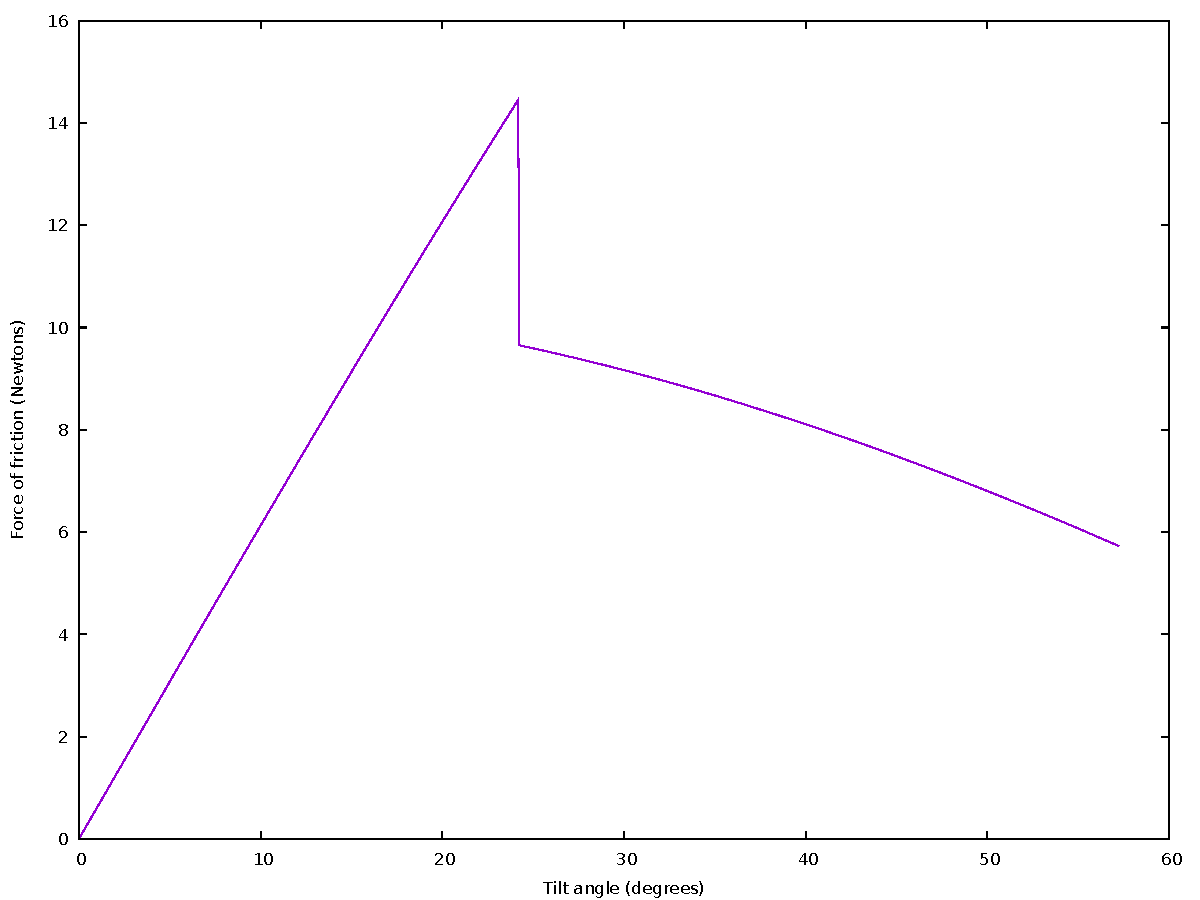
\includegraphics[width=0.7\textwidth]{tilt.pdf}	
	
\end{center}


\begin{minipage}{0.5\textwidth}
\begin{center}
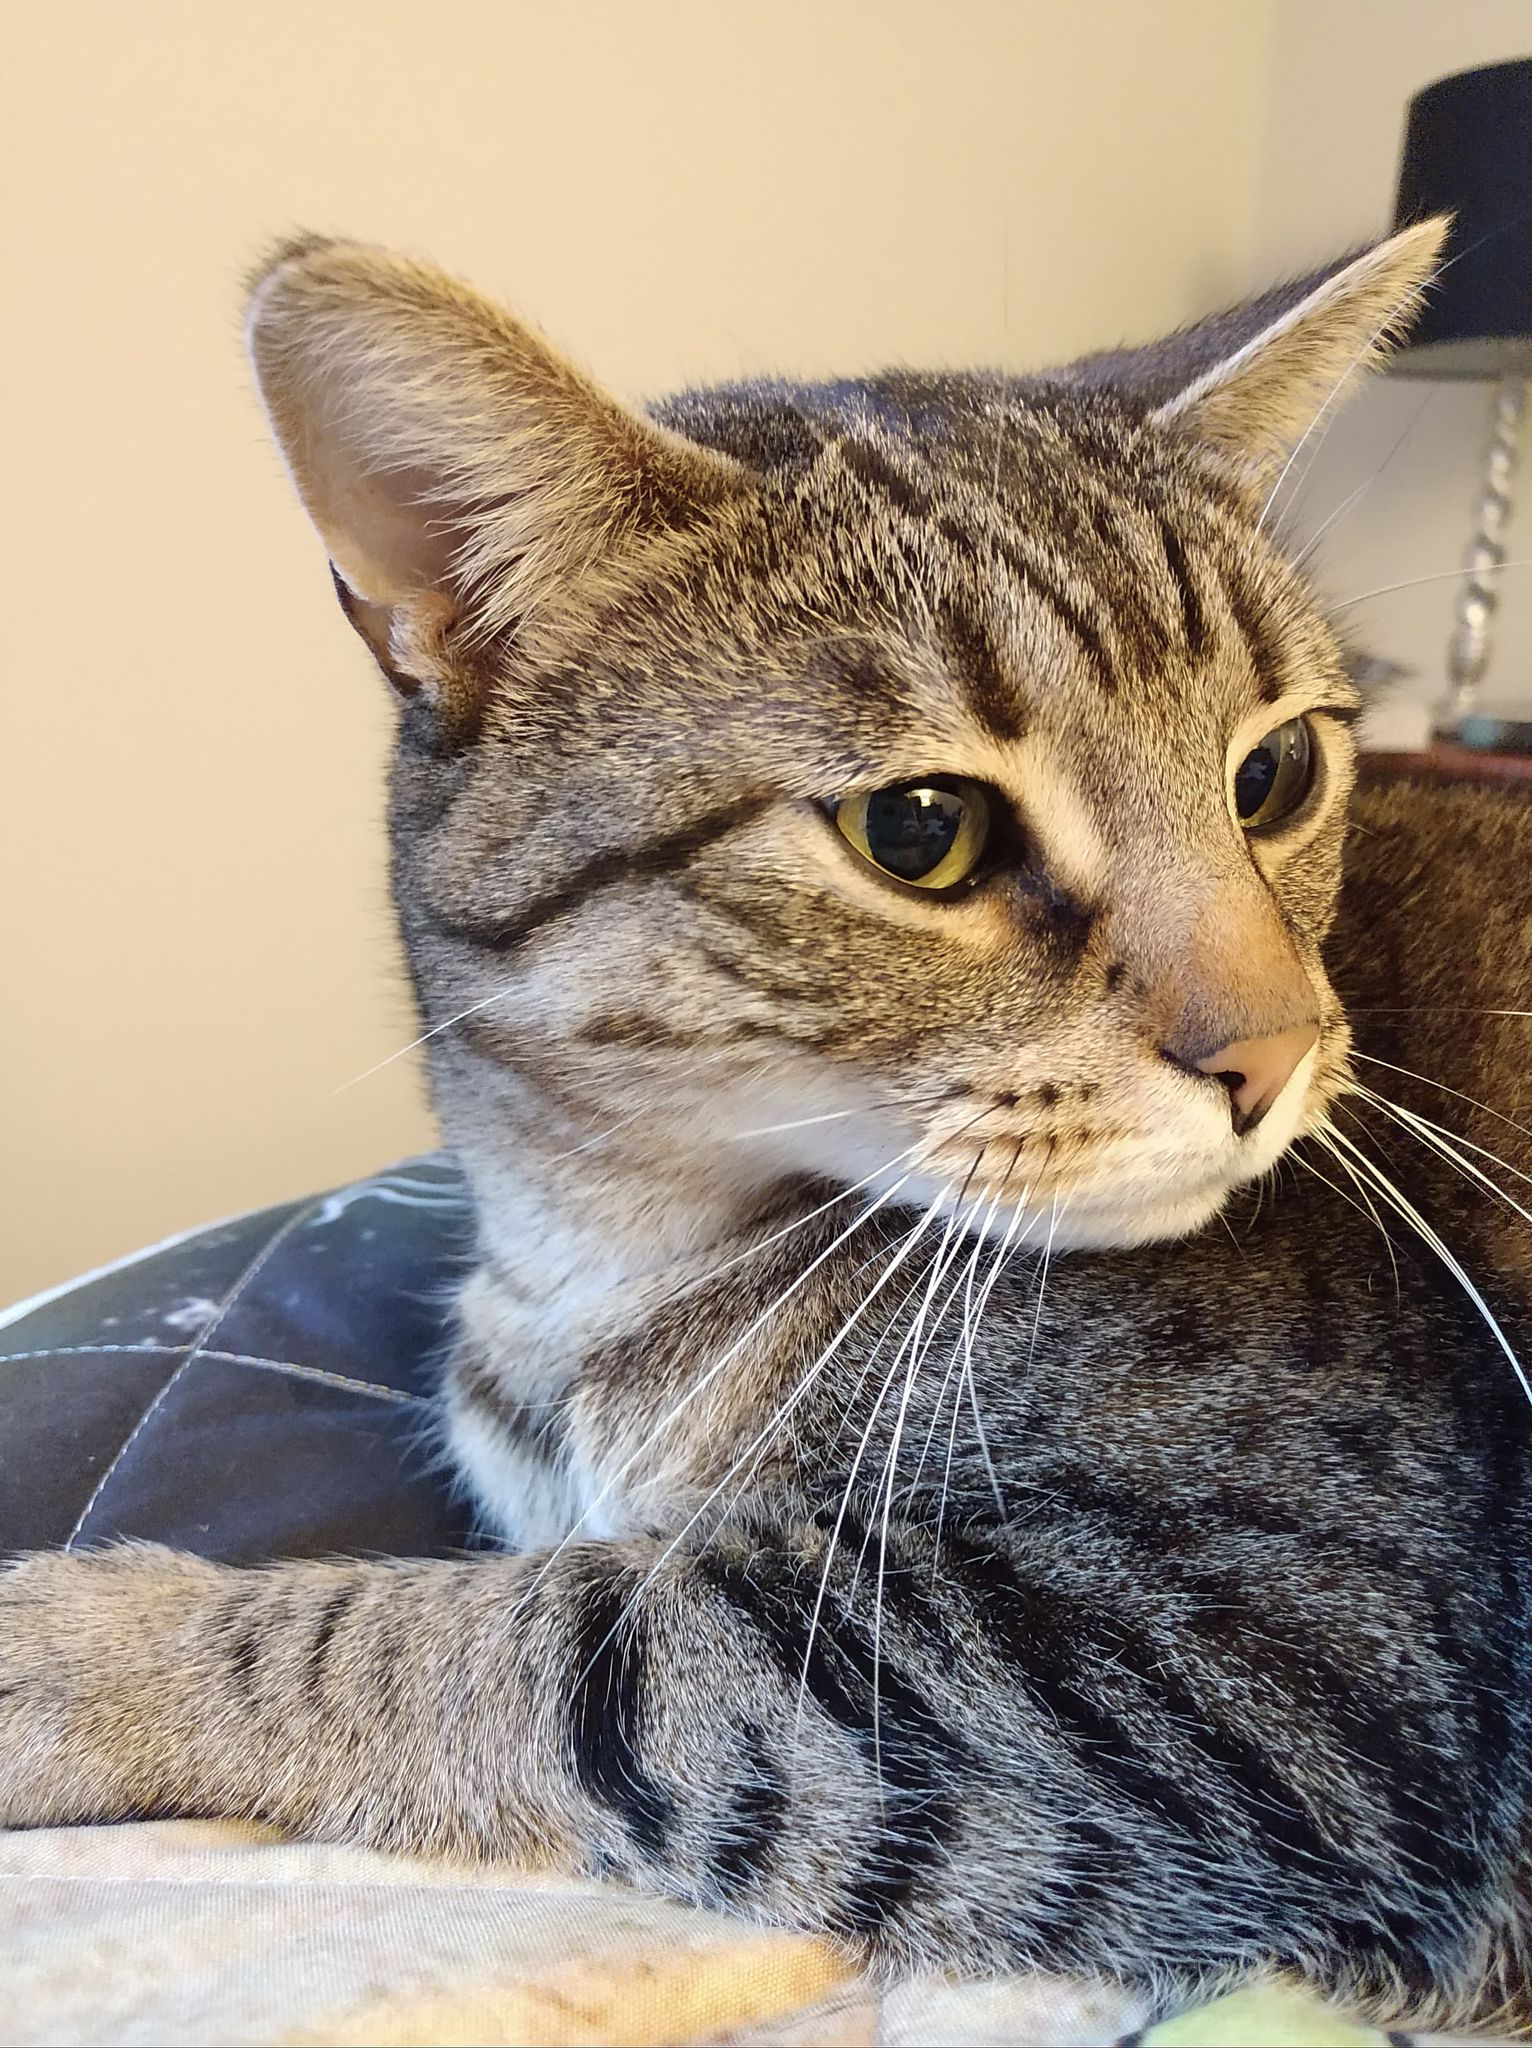
\includegraphics[width=0.5\textwidth]{matilda.jpg}

\scriptsize \it Waltzing Matilda, the three-legged wonder kitty
\end{center}
\end{minipage}
\begin{minipage}{0.5\textwidth}
	\begin{center}
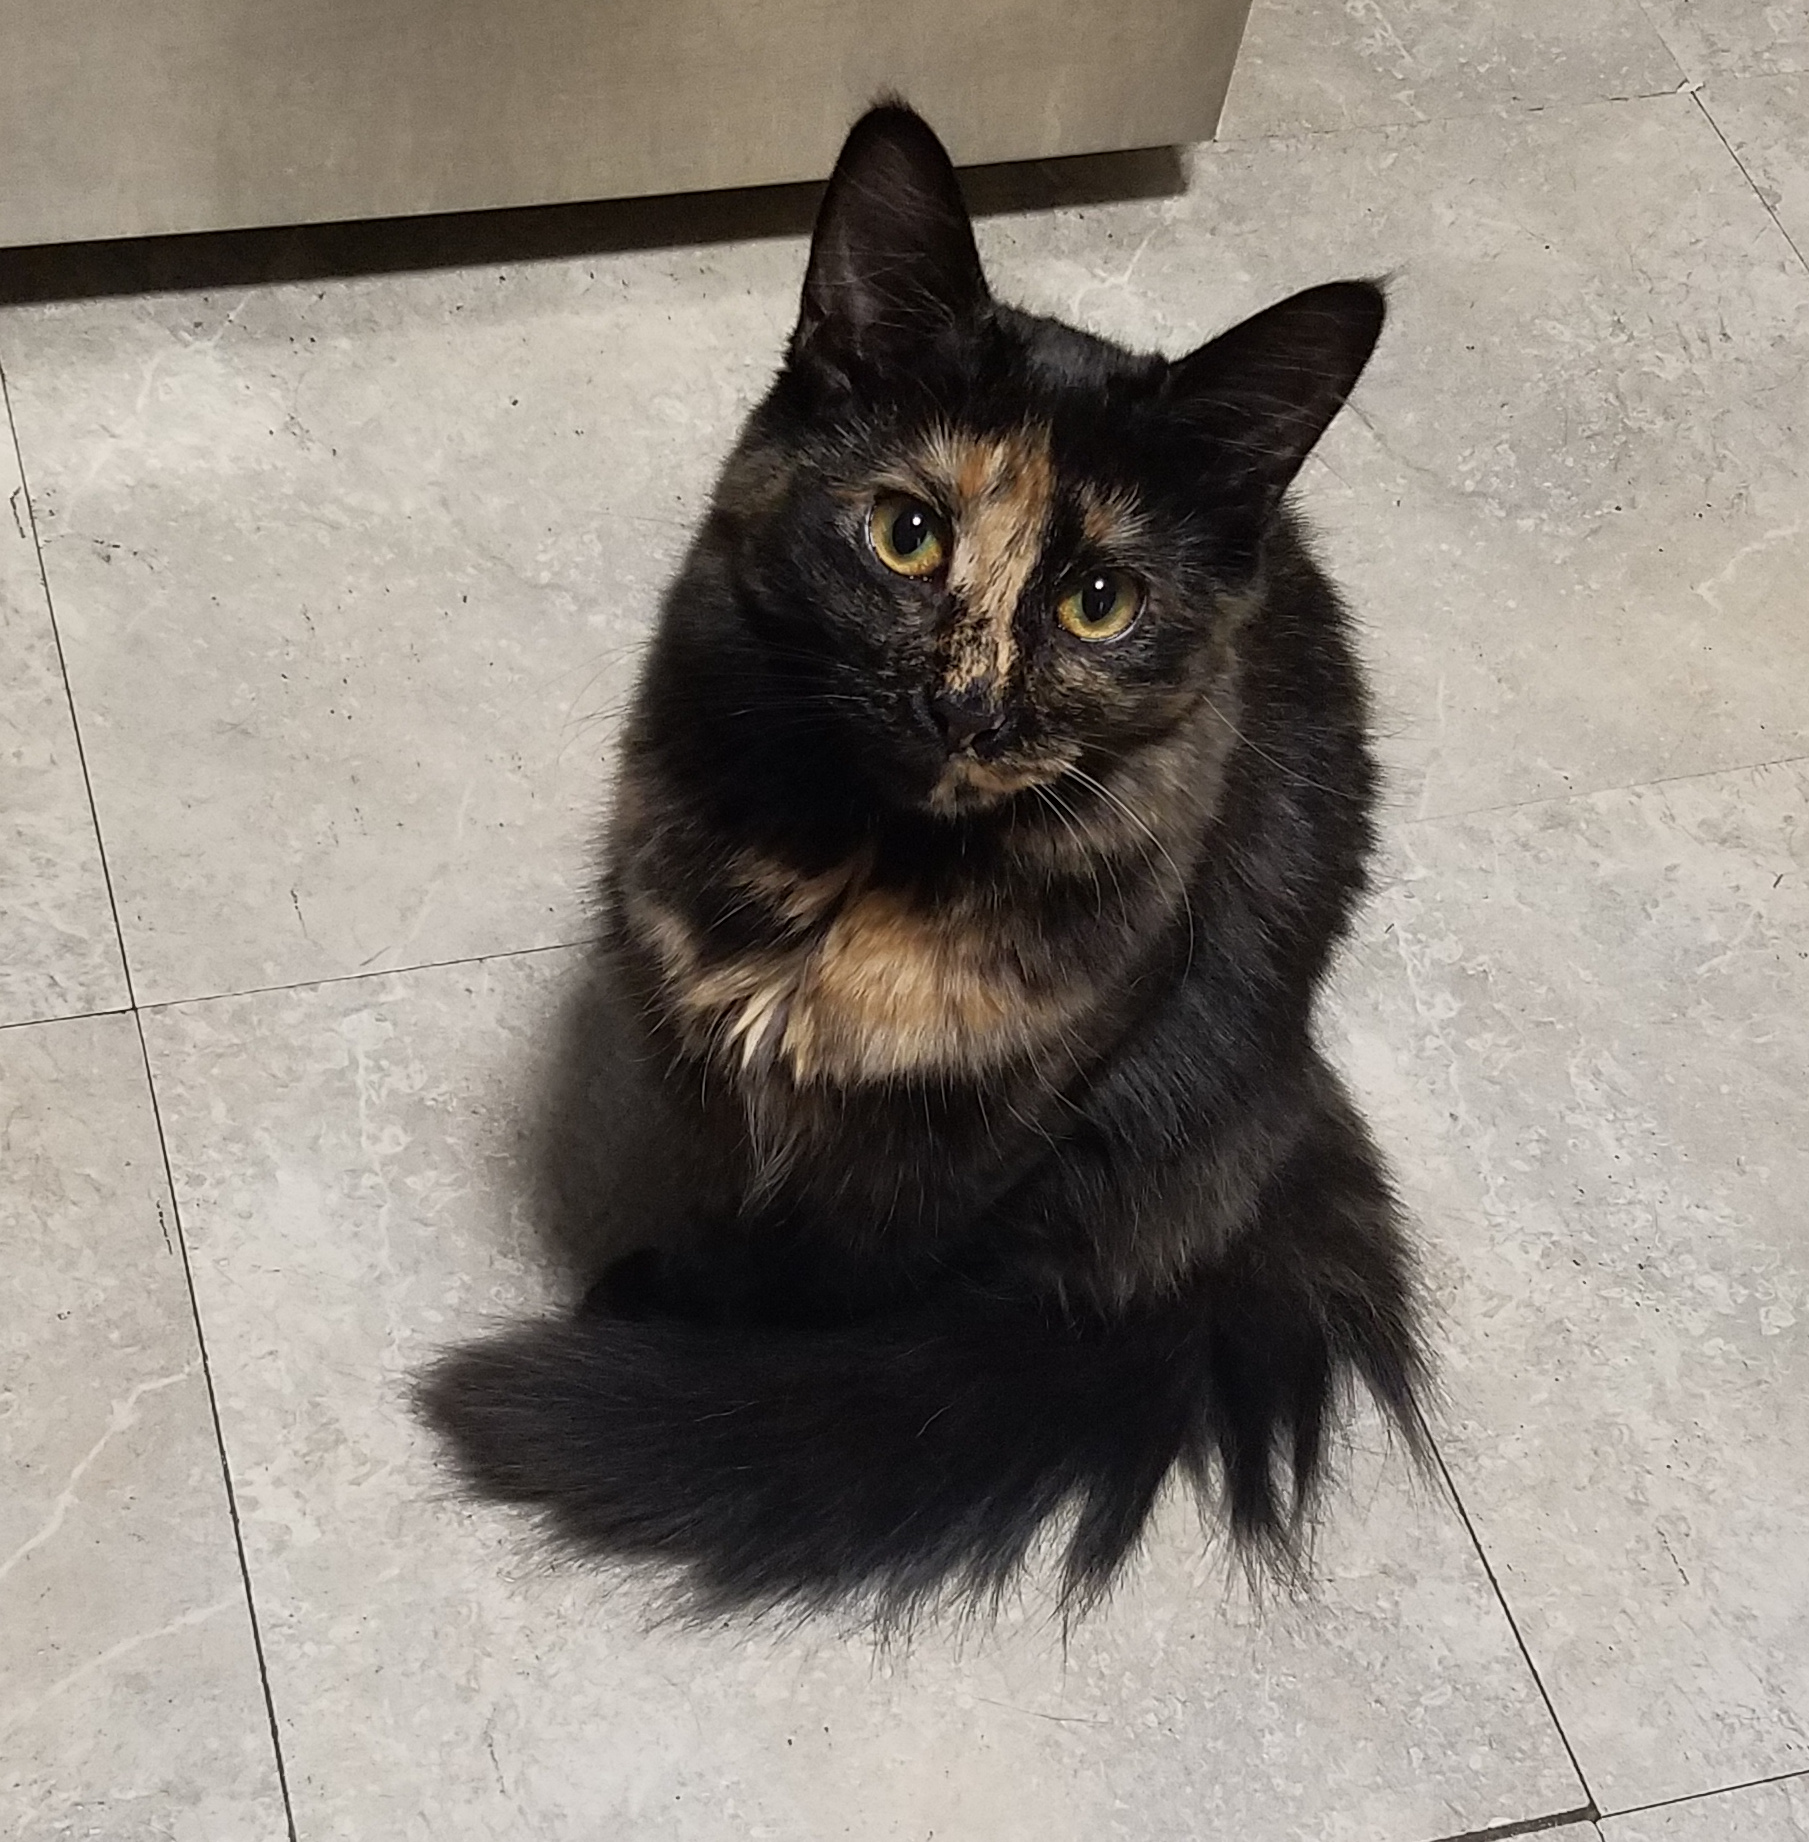
\includegraphics[width=0.7\textwidth]{lucky.jpg}

\scriptsize \it Lucky, a very fluffy fuzzy troublemaker, sent in by Lumberjack from the class Discord server
\end{center}
\end{minipage}


\newpage

You already met our previous head TA Ohana Benevides' dog Rum. But she has another dog, Quanta, who is much smaller.

Rum has mass $m_R$ and coefficient of static friction $\mu_s$; Quanta and her sled have mass $m_Q$ and coefficient of kinetic friction $\mu_k$. (Remember that traction is just a special kind of static friction, and so the maximum traction force that Rum can exert is also equal to $\mu_s F_N$.)

Rum is trying to pull Quanta and her sled up a hill sloping up at an angle $\theta$ at a constant speed. In this problem, you'll solve for the
steepest hill that they can climb.

a) Draw a cartoon of the problem, and choose a coordinate system. 

\vspace{2in}

b) Draw a force diagram for each dog. 

\vspace{3in}
\newpage
c) Write down Newton's second law in both directions -- that is, $\sum F_x = ma_x$ and $\sum F_y = ma_y$ -- 
in both directions.

\vspace{2in}
d) This will result in four equations. Plug in things that you know. (What do you know about their accelerations?) This will result in four equations with 
four unknowns. What is true about the traction force on Rum when he's climbing the steepest hill that he can?
Underneath each equation, identify the physical meaning of each term (i.e. ``component of Quanta's weight parallel to the slope''). 

\vspace{3.5in}

e) Discuss how you'd do the algebra to solve these equations; if you have time, work on doing so.

\end{document}
